\section{Experiments}

We evaluate \textit{\lowrank} on pre-training and fine-tuning tasks for LLMs. All experiments are conducted on a single node with 8 NVIDIA A100 GPUs to leverage high-performance computing capabilities, yet stay within reasonable limits.

\subsection{Pre-training on the C4 Dataset}

To assess the effectiveness of \textit{\lowrank}, we apply it to pre-train LLaMA-based language models of sizes ranging from 60 million to 1.1 billion parameters, on the C4 dataset. The C4 dataset is a colossal, cleaned version of the Common Crawl Corpus, primarily intended for pre-training language models and word representations \citep{raffelExploringLimitsTransfer2020}. It provides a diverse and extensive corpus, making it suitable for evaluating pre-training methods in realistic scenarios.

We adopt the experimental setup from \citet{lialinReLoRAHighRankTraining2023}, utilizing a LLaMA-based\footnote[2]{LLaMA materials in our paper are subject to the LLaMA community license.} architecture with RMSNorm and SwiGLU activations \citep{shazeerGLUVariantsImprove2020,touvronLlamaOpenFoundation2023}. We maintain the same set of hyperparameters for each model size across all methods, except for the learning rate, which is tuned individually to ensure optimal performance. All experiments use the BF16 format to reduce memory usage without compromising computational efficiency, the same computational budget and the best validation perplexity is reported.

\begin{figure}[ht]
    \centering
    \vspace{-2.5mm}
    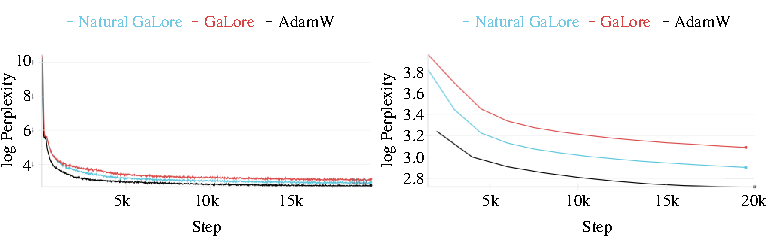
\includegraphics[width=\linewidth]{figures/train_and_validate.pdf}
    \vspace{-5.5mm}
    \caption{\small{Training and Validation log Perplexity for Llama 1.1B
    }}
    \vspace{-5mm}
    \label{fig:train_loss}
\end{figure}


\begin{table*}[ht]
    \centering
    \caption{\small{Comparison of \textit{\lowrank} with other low-rank algorithms on pre-training various sizes of LLaMA models on the C4 dataset. Validation log perplexity is reported (averaged over 5 runs), along with a memory estimate (in gigabytes) of the total parameters and optimizer states based on BF16 format.}}
    \label{tab:lora_compare_llama}
    \begin{tabular}{lcccc}
    \toprule
                     & \textbf{60M} & \textbf{130M} & \textbf{350M} & \textbf{1.1B} \\
    \midrule
    Full-Rank        & 3.52 (0.36G) & 3.22 (0.76G) & 2.93 (2.06G) & 2.72 (7.80G) \\
    \midrule
    \textit{\lowrank} & \textbf{3.53} (0.24G) & \textbf{3.22} (0.52G) & \textbf{2.93} (1.22G) & \textbf{2.80} (4.38G) \\
    GaLore           & 3.56 (0.24G) & 3.24 (0.52G) & 2.95 (1.22G) & 2.90 (4.38G) \\
    Low-Rank         & 4.35 (0.26G) & 3.82 (0.54G) & 3.62 (1.08G) & 4.96 (3.57G) \\
    LoRA             & 3.55 (0.36G) & 3.52 (0.80G) & 3.24 (1.76G) & 2.96 (6.17G) \\
    ReLoRA           & 3.61 (0.36G) & 3.38 (0.80G) & 3.37 (1.76G) & 2.91 (6.17G) \\
    \bottomrule
    Rank $r / d_{\text{model}}$ & 128 / 256 & 256 / 768 & 256 / 1024 & 512 / 2048 \\
    Training Tokens  & 1.1B & 2.2B & 6.4B & 13.1B \\
    \bottomrule
    \end{tabular}
\end{table*}

Table~\ref{tab:lora_compare_llama} presents the validation perplexity and memory consumption for models trained with different methods and Figure~\ref{fig:train_loss} shows the training run for the Llama 1.1B model. Our proposed \textit{\lowrank} consistently outperforms GaLore \citep{zhao2024galore} across all model sizes, achieving validation perplexities closer to the full-rank baseline while maintaining significant memory savings. Furthermore, \textit{\lowrank} exhibits lower perplexities and greater memory consumption compared to other low-rank adaptation methods like LoRA and ReLoRA, due to their less efficient use of low-rank structures and the need for additional optimizer states.

\vspace{-2mm}

\subsection{Fine-Tuning RoBERTa-Base on the GLUE Benchmark}

To further evaluate the effectiveness of \textit{\lowrank}, we conduct experiments on the General Language Understanding Evaluation (GLUE) benchmark using the pre-trained RoBERTa-Base model. The GLUE benchmark is a collection of nine natural language understanding tasks, including single-sentence tasks like CoLA \citep{warstadt2019neural}, similarity and paraphrase tasks like MRPC \citep{dolan2005automatically} and STS-B \citep{cer2017semeval}, and inference tasks like RTE \citep{dagan2005pascal}, MNLI \citep{williams2018broad}, and QNLI \citep{rajpurkar2016squad}. This benchmark is widely used to assess the performance of language models on diverse linguistic phenomena.

In our experiments, we fine-tune the RoBERTa-Base model using \textit{\lowrank} and compare its performance with full fine-tuning and LoRA \citep{huLoRALowRankAdaptation2021}. We focus on memory-efficient fine-tuning methods to reduce the computational footprint while maintaining high performance. For each method, we report the average score across all GLUE tasks and individual task scores.

We use the same training hyperparameters across all methods for a fair comparison. The batch size is 32, and we fine-tuned each model for three epochs. The learning rate is selected from \{1e-5, 2e-5, 3e-5\} based on the best validation performance for each task. For \textit{\lowrank} and LoRA, we experiment with rank values of 4 and 8 to study the trade-off between performance and memory efficiency.

Table~\ref{tab:fine_tuning} presents the results of our experiments. \textit{\lowrank} consistently achieves comparable or better performance than LoRA across most tasks while using less memory. Precisely, with a rank of 4, \textit{\lowrank} attains an average score of \textbf{86.05}, closely matching the complete fine-tuning baseline of 86.28 and outperforming LoRA's average score of 85.61. This demonstrates that \textit{\lowrank} can effectively fine-tune large models with reduced memory consumption without sacrificing performance.

\begin{table}[ht]
    \caption{\small{Evaluating \textit{\lowrank} for memory-efficient fine-tuning on the GLUE benchmark using pre-trained RoBERTa-Base. We report the average score of all tasks. Memory consumption is reported in millions of parameters (M).}}
    \label{tab:fine_tuning}
    \centering
    \resizebox{\linewidth}{!}{%
    \begin{tabular}{l|c|cccccccc|c}
    \toprule
               & \textbf{Memory} & \textbf{CoLA} & \textbf{STS-B} & \textbf{MRPC} & \textbf{RTE} & \textbf{SST-2} & \textbf{MNLI} & \textbf{QNLI} & \textbf{QQP} & \textbf{Avg} \\
    \midrule
    Full Fine-Tuning & 747M & 62.24 & 90.92 & 91.30 & 79.42 & 94.57 & 87.18 & 92.33 & 92.28 & 86.28 \\
    \midrule
    \textbf{\textit{\lowrank} (rank=4)} & 253M & 61.50 & \textbf{90.80} & \textbf{92.10} & \textbf{79.50} & \textbf{94.20} & \textbf{87.05} & \textbf{92.30} & 91.15 & \textbf{86.05} \\
    GaLore (rank=4) & 253M & 60.35 & 90.73 & 92.25 & 79.42 & 94.04 & 87.00 & 92.24 & 91.06 & 85.89 \\
    LoRA (rank=4) & 257M & \textbf{61.38} & 90.57 & 91.07 & 78.70  & 92.89 & 86.82 & 92.18 & \textbf{91.29} & 85.61 \\
    \midrule
    \textbf{\textit{\lowrank} (rank=8)} & 257M & 61.70 & \textbf{90.90} & \textbf{92.25} & \textbf{79.80} & \textbf{94.40} & \textbf{87.20} & \textbf{92.35} & \textbf{91.25} & \textbf{86.23} \\
    GaLore (rank=8) & 257M & 60.06 & 90.82 & 92.01 & 79.78 & 94.38 & 87.17 & 92.20 & 91.11 & 85.94 \\
    LoRA (rank=8) & 264M & \textbf{61.83} & 90.80 & 91.90 & 79.06  & 93.46 & 86.94 & 92.25 & 91.22 & 85.93 \\
    \bottomrule
    \end{tabular}
    }
    \vskip -0.1in
\end{table}


\vspace{-2mm}

\subsection{Fine-Tuning TinyLlama 1.1B for Function Calling in Advanced Agentic Systems}

Advanced Agentic Systems (AAS) require language models that can understand and generate code snippets to integrate various tools and APIs, fulfilling user queries through function-calling. We utilize the TinyAgent framework, which provides an end-to-end pipeline for training and deploying task-specific LLM agents capable of efficient and accurate function-calling \citep{erdogan2024tinyagent} to drive agentic systems at the edge.

Given a natural language query, the LLM agent must generate a sequence of pre-defined function-calls that accomplish the desired tasks. The challenge lies in determining the appropriate arguments, to call the correct functions, in the right order while respecting interdependencies among the functions.

LLMCompiler \citet{kim2023llmcompiler}, is a framework that enables language models to perform function-calling by first generating a function-calling plan, which includes the required functions and arguments. The LLMCompiler then compiles this plan into an executable sequence of function-calls. The critical aspect is training the model to produce a function-calling plan with the correct syntax and dependencies.

The off-the-shelf pre-trained TinyLlama 1.1B (instruct-32k) model performs poorly on this task. The model generates incorrect sets of functions, hallucinated function names, fails to respect dependencies, and passes arguments incorrectly. This underperformance is expected, as the model was initially trained on datasets like SlimPajama and StarCoder, which are not specific to function-calling tasks. To address this, we follow the TinyAgent framework \citep{erdogan2024tinyagent} and fine-tune the TinyLlama 1.1B model on a high-quality, curated dataset designed for function-calling.

\paragraph{TinyAgent Dataset}

The TinyAgent dataset \citep{erdogan2024tinyagent} is a meticulously curated collection aimed at building a local agentic system for function-calling on Apple MacBooks for day-to-day tasks. It contains 40K examples of natural language queries and corresponding function-calling plans. The dataset is divided into 38K training examples, 1K validation examples, and 1K test examples. It encompasses 16 tasks, including Email, Contacts, SMS, Calendar, Notes, Reminders, File Management and Zoom Meetings. Each task has predefined scripts that the model needs to generate. The dataset is intentionally challenging, requiring the model to understand dependencies between function-calls and the arguments to be passed.

\paragraph{Fine-Tuning Procedure}

We fine-tune the TinyLlama 1.1B model on the TinyAgent dataset for three epochs using a batch size of 32. The learning rate is set to \(7 \times 10^{-5}\). After each epoch, the model is evaluated on the validation set, and the best-performing model is selected based on validation performance to be evaluated on the test set.

During fine-tuning, the prompt includes descriptions of the ground truth functions and irrelevant functions serving as negative samples. This strategy encourages the model to learn to select the correct functions rather than merely memorizing the ground truth. Additionally, several in-context examples demonstrate how queries are translated into function-calling plans. These examples are selected using a Retrieval-Augmented Generation (RAG) process based on the user's query from the training data and a DeBERTa-v3-small model \citep{he2021debertav3} fine-tuned for multi-label classification for retrieval among the 16 tools.

The training objective is then to maximize the accuracy of the generated function-calling plans. Success is defined by the model generating the correct plan with the proper set of function-calls, correct arguments, and the appropriate order of function-calls. Verifying the selection of the correct set of functions involves straightforward set comparison. However, ensuring the correctness of arguments and the order of function-calls is more complex and requires constructing the associated Directed Acyclic Graph to check for equality.

\paragraph{Results and Discussion}

\begin{table*}[ht]
\vspace{-3mm}
\caption{
Latency, size, and success rate of TinyAgent models before and after quantization. Latency is the end-to-end latency of the function calling planner, including the prompt processing time and generation.}
\vspace{-1mm}
\begin{center}
\small{
\setlength{\tabcolsep}{6pt}{
\begin{tabular}{c|c|c|c|c}
\toprule
Model &	Weight Precision &	Latency (seconds)	& Model Size (GB)	& Success Rate (\%) \\
\midrule
GPT-3.5 & Unknown & 3.2 & Unknown & 65.04 \\
GPT-4-Turbo & Unknown & 3.9 & Unknown & 79.08 \\
\midrule
\multirow{2}{*}{TinyAgent-1.1B} & 16-bit (\textit{\lowrank}) & 3.9 & 2.2 & \textbf{83.09} \\
& 16-bit (LoRA) & 3.9 & 2.2 & 80.06 \\
\midrule
\multirow{1}{*}{TinyAgent-7B} & 16-bit \citep{erdogan2024tinyagent} & 19.5 & 14.5 & 84.95 \\
\bottomrule
\end{tabular}
}
}
\end{center}
\label{table:t2}
\end{table*}




After fine-tuning, the TinyLlama 1.1B model's success rate on the test set improved significantly. Table~\ref{table:t2} presents the latency, model size, and success rate of various models on the TinyAgent dataset. As shown, \textit{\lowrank} improves the success rate of the 1.1B model from 80.06\% (16-bit LoRA) to \textbf{83.09\%}, also surpassing GPT-4-Turbo by 4\% and approaching the performance of the larger TinyAgent-7B model, which achieves 84.95\%.

These results demonstrate that \textit{\lowrank} not only enhances the performance of smaller models like the 1.1B parameter TinyLlama but also makes them competitive with significantly larger models. By efficiently incorporating second-order information through low-rank natural gradient updates, \textit{\lowrank} enables smaller models to achieve higher accuracy without additional memory overhead.